\documentclass[nobib]{tufte-handout}

\usepackage{amssymb}
\usepackage{hyperref}
\usepackage{pgfplots}
\usepackage[activate={true,nocompatibility},final,tracking=true,kerning=true,spacing=true,factor=1100,stretch=10,shrink=10]{microtype}
\usepackage{color}
\usepackage{steinmetz}
\usepackage{placeins}
\usepackage{marginfix}
\usepackage{array}
\usepackage{tikz}
\usetikzlibrary{arrows.meta, positioning, shapes.geometric}
\usepackage{circuitikz}
\usepackage{amsmath}
\usepackage{amsthm}
\usepackage{booktabs}
\usepackage{listings}
\usepackage[edges]{forest}
\usepackage{caption}
\usepackage[T1]{fontenc}
\usepackage{lmodern}
\usepackage{units}
\usepackage{fancyvrb}
\usepackage{multicol}
\DeclareCaptionFont{white}{\color{white}}
\DeclareCaptionFormat{listing}{\colorbox{gray}{\parbox{\textwidth}{#1#2#3}}}
\captionsetup[lstlisting]{format=listing,labelfont=white,textfont=white}

% Set up the images/graphics package
\usepackage{graphicx}
\setkeys{Gin}{width=\linewidth,totalheight=\textheight,keepaspectratio}
\graphicspath{{.}}

\title{Notes for ECE 36200 - Microprocessor Systems And Interfacing}
\author{Zeke Ulrich}
\date{\today} 

\fvset{fontsize=\normalsize}
\usetikzlibrary{shapes}
\usetikzlibrary{positioning}

% For finite state machines 
\usetikzlibrary{automata} % Import library for drawing automata
\usetikzlibrary{positioning} % ...positioning nodes
\usetikzlibrary{arrows} % ...customizing arrows
\tikzset{node distance=2.5cm, % Minimum distance between two nodes. Change if necessary.
    every state/.style={ % Sets the properties for each state
    semithick,
    fill=gray!10},
    initial text={}, % No label on start arrow
    double distance=2pt, % Adjust appearance of accept states
    every edge/.style={ % Sets the properties for each transition
    draw,
    ->,>=stealth', % Makes edges directed with bold arrowheads
    auto,
    semithick}}
\let\epsilon\varepsilon

% These commands are used to pretty-print LaTeX commands
\newcommand{\doccmd}[1]{\texttt{\textbackslash#1}}% command name -- adds backslash automatically
\newcommand{\docopt}[1]{\ensuremath{\langle}\textrm{\textit{#1}}\ensuremath{\rangle}}% optional command argument
\newcommand{\docarg}[1]{\textrm{\textit{#1}}}% (required) command argument
\newenvironment{docspec}{\begin{quote}\noindent}{\end{quote}}% command specification environment
\newcommand{\docenv}[1]{\textsf{#1}}% environment name
\newcommand{\docpkg}[1]{\texttt{#1}}% package name
\newcommand{\doccls}[1]{\texttt{#1}}% document class name
\newcommand{\docclsopt}[1]{\texttt{#1}}% document class option name

% Define a custom command for definitions and biconditional
\newcommand{\defn}[2]{\noindent\textbf{#1}:\ #2}
\let\biconditional\leftrightarrow

\begin{document}

\maketitle

\tableofcontents

\section{Course Description}
An introduction to basic computer organization, microprocessor instruction sets, assembly language programming, and microcontroller peripherals.
\pagebreak

\section{GPIO}
\emph{General Purpose Input/Output} (GPIO)

Input/output (I/O) is the interface between our digital microcontroller (MCU) and the rest of the world.
Each MCU has pins which its software uses to read input and write output.

Some pins are general purpose I/O, but some are used to power the MCU (VDD, GND) and some pins are
special (oscillator, clock pins), can to analog to digital I/O or vice versa, or more complex digital I/O (SPI, I2C, UART).

Digital input reads the pin to check if an external voltage is applied. Digital output drives the voltage on the pin. More advanced circuity performs
digital-to-analog conversion (DAC) or analog-to-digital (ADC).

The layout of every GPIO pin port looks like Figure \ref{fig:gpio}

\begin{figure}
    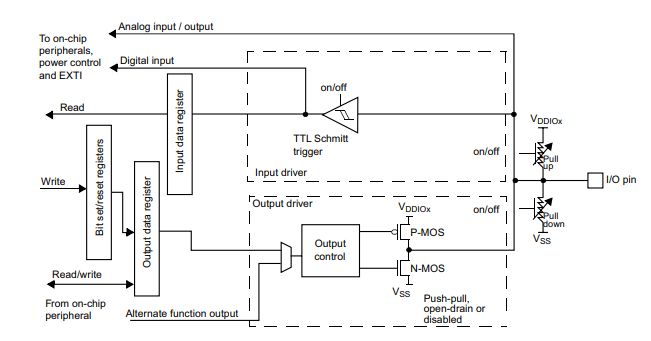
\includegraphics{images/gpio.png}
    \caption{GPIO Layout}
    \label{fig:gpio}
\end{figure}

Each MCU has multiple GPIO ports A, B, etc. Each port has multiple
GPIO bits (typically 8).

\subsection{Output}

The way output works is that an output bit is written
into the Output Data Register (ODR). Then the output driver
reads the ODR and drives the pin either high or low depending on
the value of the ODR bit. The voltage then appears on the I/O pin.

The GPIO can be configured as either read or write, output mode of push-pull
or open drain, output speed, and more.

In push-pull mode, we have need of a buffer to increase the output voltage
of the MCU so that when the output of the software is 1 the output
of the GPIO pin is VCC. This is accomplished with two NOT gates. If the software
write a 1, then the controller outputs a 0 to a NOT gate, which pulls the
output pin to 1. Basically, in push-pull mode the MCU actively drives the pin
low for 0 or high for 1.

In open drain mode, the MCU drives the output to low, but floats in 1. That is
the GPIO pin can be 0 volts, but it cannot be VCC. Basically, it can actively
drive a pin low for 0, but leaves the pin floating for 1. Open drain mode
is useful when there are multiple outputs. Two output pins can be tied together,
which isn't possible with push-pull outputs because one could be high and one low,
causing a short circuit. Thus, all tied pins must be open drain to avoid short circuits.
Any one of them can drive the shared output low, while a pull-up resistor passively
pulls the wire up to high when no MCU is driving it to low.
\marginnote{This is how I23 works. More details to follow in the unit of I2C.}

Another configurable is output speed, the speed of voltage rising and falling.
A faster GPIO is good for fast communication, but higher speed increases
electromagnetic interference and power consumption.

A related concept is slew rate, defined as
\begin{equation}
    \max(\frac{\Delta V}{\Delta t})
\end{equation}

\subsection{Input}

With input, an external circuit applies a voltage to the I/O pin.
The input driver converts the voltage to either 1 or 0. The input
is then sampled into the Input Data Register (IDR) every clock cycle.

In real life, the input voltage is noisy and messy. We add a Schmitt trigger
to smooth it, reduce noise, and increase the slew rate to make it suitable
for our digital circuit. Recall that a Schmitt trigger is just a buffer
that is immune to oscillating issues because it has a low and high threshold.
When the input signal crosses the high threshold, the output of the Schmitt
trigger is high. It stays high until the input signal crosses the low threshold,
at which point the output of the Schmitt trigger goes low.

Electricity in the real world is unfortunately messy.
Consider the circuit in Figure \ref{fig:faulty-led-circuit}.

\begin{figure}[h]
    \centering
    \begin{circuitikz}[american]
        % VDD power supply
        \draw (1.5,2.5) node[buffer] (mybuffer) {};
        \node at (0,4) {VDD};
        \draw (0,4) to[short] (0,3.5);

        % Switch
        \draw (0,3.5) to[nos] (0,2.5);
        \node at (-0.5,3) {};

        % Buffer (simple triangle)
        \draw (0,2.5) to[short] (1,2.5);
        \draw (2,2.5) to[short] (2.5,2.5);

        % Resistor
        \draw (2.5,2.5) to[R, l=$R$] (4,2.5);

        % LED
        \draw (4,2.5) to[led] (4,1);

        % Ground
        \draw (4,1) to[short] (4,0.5);
        \node[ground] at (4,0.5) {};
    \end{circuitikz}
    \caption{Faulty LED Control Circuit}
    \label{fig:faulty-led-circuit}
\end{figure}

You would expect that the circuit turns off when
the switch is open. However, the input to the buffer
would be floating, so the output of the buffer is unpredictable.

We can remedy this by adding a pull-down resistor, as in Figure
\ref{fig:led-circuit}.

\begin{figure}[h]
    \centering
    \begin{circuitikz}[american]
        % VDD power supply
        \draw (1.5,2.5) node[buffer] (mybuffer) {};
        \node at (0,4) {VDD};
        \draw (0,4) to[short] (0,3.5);

        % Switch
        \draw (0,3.5) to[nos] (0,2.5);
        \node at (-0.5,3) {};

        % Buffer (simple triangle)
        \draw (0,2.5) to[short] (1,2.5);
        \draw (2,2.5) to[short] (2.5,2.5);

        % Resistor
        \draw (2.5,2.5) to[R] (4,2.5);

        % LED
        \draw (4,2.5) to[led] (4,1);

        % Ground
        \draw (4,1) to[short] (4,0.5);
        \node[ground] at (4,0.5) {};

        % Pull-down Resistor
        \draw (0.5,2.5) to[R] (0.5,0);
        \node[ground] at (0.5,0) {};
    \end{circuitikz}
    \caption{LED Control Circuit}
    \label{fig:led-circuit}
\end{figure}

Pins face a similar issue. A floating pin's voltage is unknown.
We need to add a pull-up or pull-down resistor so that when the
voltage isn't actively being driven low or high then the pin is
at a known voltage. The resistors have to be weaker than however
the pins are being driven, or the pin would always be high/low,
but if it's too weak then the pin will be slow and unresponsive.

Many MCUs have on-chip PU/PD resistors, which are software configurable.
Off-chip PU/PD can also be on the PCB instead, in which case it is
not configurable.

We have two options or using software to set up a pin.
\begin{itemize}
    \item Port-mapped I/O, which uses special instructions in the processor
          where every device is assigned a unique port number (used in x86).
    \item Memory-mapped I/O, which has special addresses which can be read
          from or written to in order to perform I/O.
\end{itemize}
This is true for all on-chip modules, not just GPIO.

\subsection{Memory-mapped I/O}
If we have a 32-bit CPU, each address is 1 byte and there are up
to 4 GBs of addressable memory in a 32 bit system.
\marginnote{Most modern computers are 64-bit, but MCUs are still
    mainly 32-bit.}
MCUs have limited read/write memory (less than a few MB).
Memory is \emph{byte-addressable}. Each byte has a unique address.
Addresses go from 0x00000000 to OxFFFFFFFF. The bottom sections have
on-chip flash memory, for code and data. The next sections have SRAM,
on-chip RAM, for the heap, stack, and some code. At the top is system
memory dedicated to external devices like NVIC, system timer, SCB, other
vendor-specific memory. Also in high memory (but not the highest) is
memory for external devices like SD cards. In the middle is external
RAM, off-chip memory for data. See Figure \ref{fig:mcu-memory-layout}.

\begin{figure}[h]
    \centering
    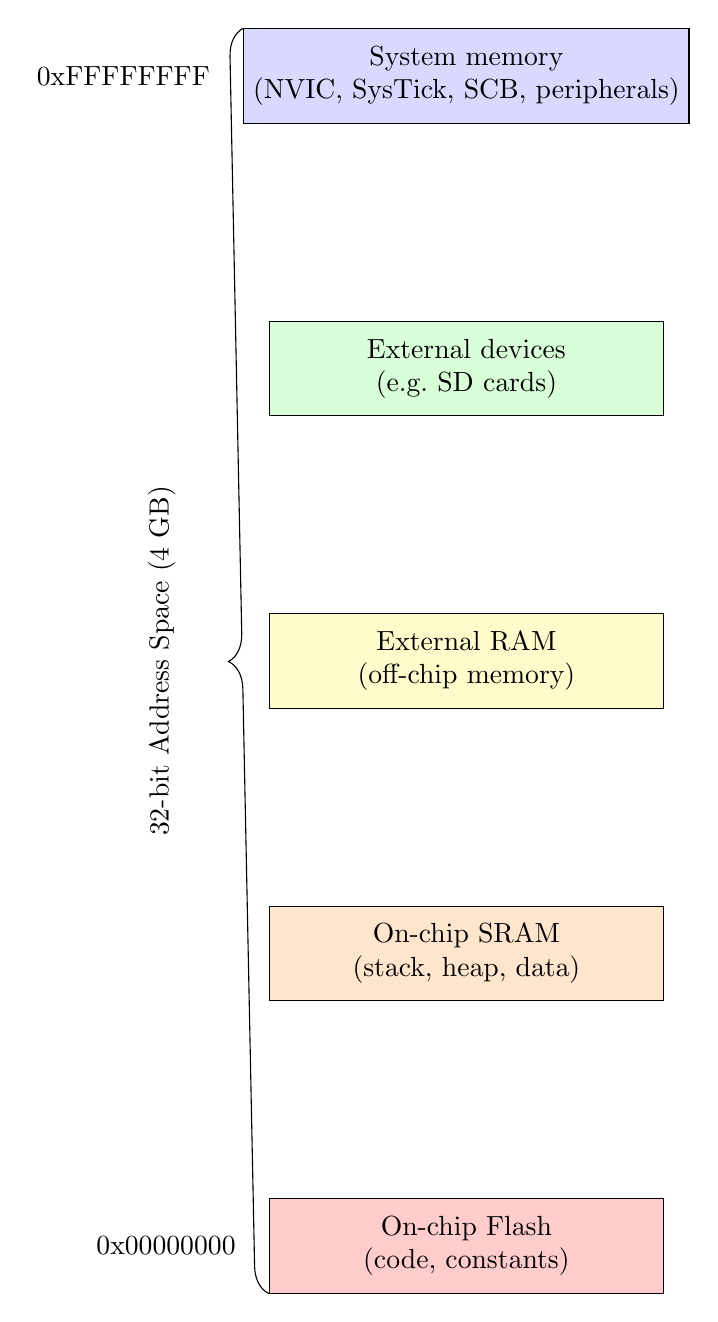
\begin{tikzpicture}[scale=1]

        % Define style
        \tikzstyle{memblock} = [rectangle, draw, minimum width=5cm, minimum height=1.2cm, align=center]

        % Blocks (top to bottom)
        \node[memblock, fill=blue!15] (system) {System memory \\ (NVIC, SysTick, SCB, peripherals)};
        \node[memblock, fill=green!15, below=of system] (extdev) {External devices \\ (e.g. SD cards)};
        \node[memblock, fill=yellow!20, below=of extdev] (extram) {External RAM \\ (off-chip memory)};
        \node[memblock, fill=orange!20, below=of extram] (sram) {On-chip SRAM \\ (stack, heap, data)};
        \node[memblock, fill=red!20, below=of sram] (flash) {On-chip Flash \\ (code, constants)};

        % Addresses
        \node[left=0.3cm of system.west] (addr1) {0xFFFFFFFF};
        \node[left=0.3cm of extdev.west] (addr2) {};
        \node[left=0.3cm of extram.west] (addr3) {};
        \node[left=0.3cm of sram.west] (addr4) {};
        \node[left=0.3cm of flash.west] (addr5) {0x00000000};

        % Brackets for column
        \draw[decorate,decoration={brace,amplitude=10pt}] (flash.south west) -- (system.north west) node[midway,xshift=-1.2cm,rotate=90] {32-bit Address Space (4 GB)};

    \end{tikzpicture}
    \caption{32-bit MCU Memory Layout}
    \label{fig:mcu-memory-layout}
\end{figure}

When the CPU needs to talk to RAM (read/write variables) it's connected
via the address bus and data bus. It reads from ROM (read-only memory).
When the CPU wants to write to the RAM, it gives an address to the address
bus and data to the data bus. The RAM looks at the address bus and if it
sees an address that belongs in RAM space, the RAM will take the data
from the data bus (if's it's a write signal) and write it at the specified
address. When the CPU wants to read it puts an address on the address bus
and signals read. The RAM sees the read signal and puts data at the specified
address on the data bus.

While RAM is read and write, ROM is read-only. The reason for this separation
is that ROM is cheaper. If you turn off your computer, anything in RAM is lost.
However, anything is ROM is non-volatile and anything flashed there will remain
even if power is lost.

GPIO modules are on the same address and data buses as the ROM and RAM. Each
periperphal has a set of control registers, including direction and data registers.
Each register has a unique memory address. If you want to write something
to the data register, get its address by looking at the data sheet, and write
there. Reading is similar. By writing a one or zero into the direction register,
you can configure the GPIO as either input or output.

To turn on an LED, for instance, we need to know what port and pin it's connected
to. We then consult the data sheet to get the addresses of the registers for
that pin and port, and then we just need to write some value to the registers.

Although the GPIO pins are not really memory, the CPU treats them like memory.
That's why this method is called memory-mapped I/O.

Memory is accessed at a minimum granularity of one byte, but typically 4.

\begin{lstlisting}
    char* controlRegisterPtr = 0x50000000;
    *controlRegisterPtr = 1;
\end{lstlisting}

\subsection{Interrupts}
A key concept in embedded systems is the need to process external stimuli,
like a button press, or when a sensor detects a change in its environment.
However, the microcontroller may already be busy executing another long
running task - maybe it's waiting on a second sensor, or its busy updating
a large display. The most efficient way to handle this issue is with
\emph{interrupts}.

An interrupt is a signal that is generated by the hardware or software
when an event occurs that needs immediate attention. Once it's fired
from an interrupt source, say a rising edge on a GPIO pin, the
interrupt signal arrives at the CPU, which - if the conditions are right
and the correct bits are set - saves what it's doing, and executes a
special function called an interrupt service routine (ISR), also called
an interrupt handler.

An interrupt is a special type of exception. Others relevant to MCUs are
faults, traps, and resets. Peripherals can raise interrupts. The
CPU can be interrupted by more than one event, each of which has its own
ISR stored in the interrupt vector table. Interrupts can be enabled or
disabled. Interrupts may have different priorities, and higher priorities
can preempt lower priorities. This means that when the CPU is servicing
one interrupt, an interrupt with a higher priority can interrupt and make
the CPU service it instead.

The flow of an interrupt is thus:
\begin{enumerate}
    \item A peripheral raises an interrupt.
    \item The CPU checks if $N$ is enabled.
    \item If $N$ is enabled, the CPU marks $N$ as pending.
    \item The CPU checks the priority of $N$ versus the current
          priority level, as it might be serving a higher priority interrupt.
    \item If the priority of $N$ is greater than the current priority
          level, then the CPU updates the current priority level to the level of
          the new interrupt and pushes the CPU state to the stack.
          It then puts the $N$th entry in the vector table into the program
          counter, a special register that keeps track of where the CPU
          is in the code. The ISR is now running.
\end{enumerate}
\begin{figure}
    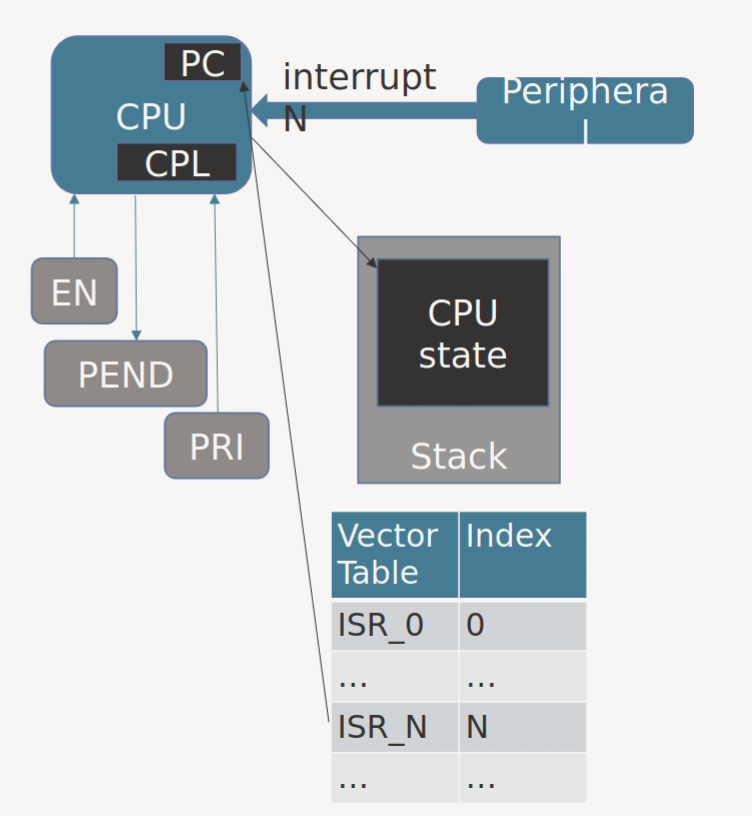
\includegraphics{images/interrupt_flow.png}
    \caption{Interrupt Flow}
    \label{fig:interrupt}
\end{figure}

\marginnote{A common exam question is "how many times was the interrupt handler interrupted?"
or "how many times was the CPU state restored?".

\subsection{Exceptions}
\section{Timers}
In MCUs, we often want a way to periodically do something or
many somethings. Every useful MCU has a hardware timer system.
A \emph{system ticker} (systick) is a special timer reserved for OS
operations, but there is always a timer subsystem outside the CPU
for general use.

The systick timer is a piece of hardware inside the MCU that generates an
systick interrupt signal at fixed intervals. Every interrupt has a dedicated
ISR to handle it, and in the case of systick the ISR is \texttt{SysTick\_Handler}.

In the ARM Cortex-M, the system timer is built into the hardware of the
CPU. Every time an IRQ is raised, the Nested Vectored Interrupt
Controller (NVIC) hardware will determine whether or not to handle the
systick interrupt.

\begin{figure}
    \centering
    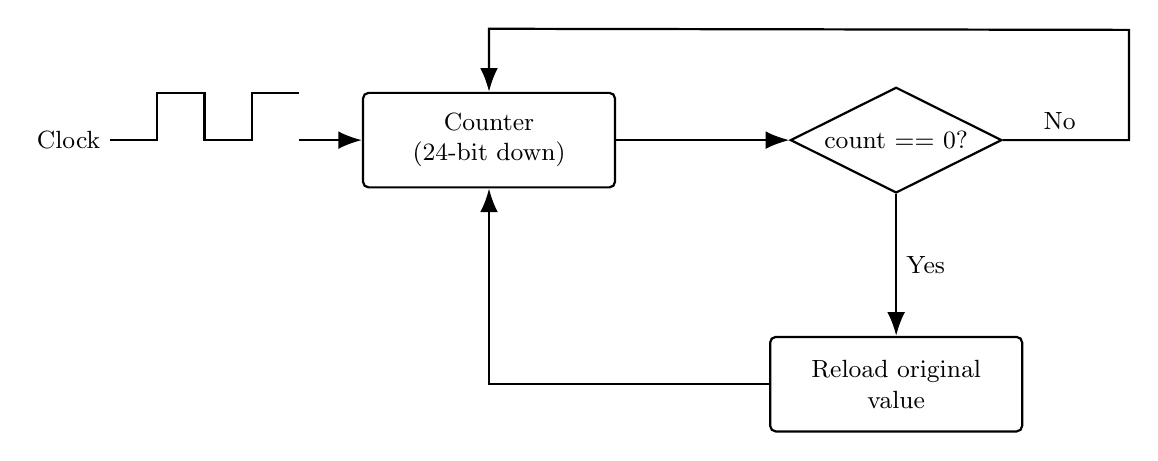
\begin{tikzpicture}[node distance=2.2cm and 2.2cm, font=\small]
        \tikzset{
        block/.style   = {draw, thick, rectangle, rounded corners=2pt, minimum width=3.2cm, minimum height=1.2cm, align=center},
        decision/.style= {draw, thick, diamond, aspect=2, inner sep=2pt, align=center},
        line/.style    = {thick, -{Latex[length=3mm]}}
        }

        % Counter and logic
        \node[block] (counter) {Counter\\(24-bit down)};
        \node[decision, right=of counter] (iszero) {count == 0?};
        \node[block, below=1.8cm of iszero] (reload) {Reload original\\value};

        % Connections
        \draw[line] (counter.east) -- (iszero.west);
        \draw[line] (iszero.east) -- ++(1.6,0) node[above, pos=0.45]{No} -- ++(0,1.4) -- ($ (counter.north) + (0,0.8) $) -- (counter.north);
        \draw[line] (iszero.south) -- node[right]{Yes} (reload.north);
        \draw[line] (reload.west) -| (counter.south);

        % Clock waveform feeding the counter
        \coordinate (clkstart) at ($(counter.west)+(-3.2,0)$);
        \node[left] at (clkstart) {Clock};
        \draw[thick]
        (clkstart)
        -- ++(0.6,0) -- ++(0,0.6) -- ++(0.6,0) -- ++(0,-0.6)
        -- ++(0.6,0) -- ++(0,0.6) -- ++(0.6,0);
        \draw[line] ($(clkstart)+(2.4,0)$) -- (counter.west);
    \end{tikzpicture}
    \caption{System Timer}
    \label{fig:systemtimerflowchart}
\end{figure}

When the counter hits zero, \texttt{COUNTFLAG} is set to 1.
The choice of clock input can vary, as most MCUs have multiple.
The clock input is ANDed with a flag to enable and disable.

For a timer, the desired interval $T$ is
\begin{equation}
    T = \frac{(\text{Prescalar} + 1) \times (\text{Reload} + 1)}{f}
\end{equation}

Let's do an example. Suppose the clock tick frequency $f$ is
80MHz and the goal is a systick
interval $s$ of 10ms. What must the reload value $R$ be?
\begin{align}
    R & = sf - 1                \\
      & = 10ms \times 80MHz - 1 \\
      & = 800000 - 1            \\
      & = 799999
\end{align}

Timers can do far more than just triggering interrupts.
They can also
\begin{itemize}
    \item Capture external events
    \item Drive certain peripherals like GPIO
    \item Output precisely timed signals
\end{itemize}
In output mode, hardware constantly compares the
counter with a value stored in the \emph{compare and capture register}
(CCR), as in figure
\ref{fig:outputmodetimer}.

\begin{figure}
    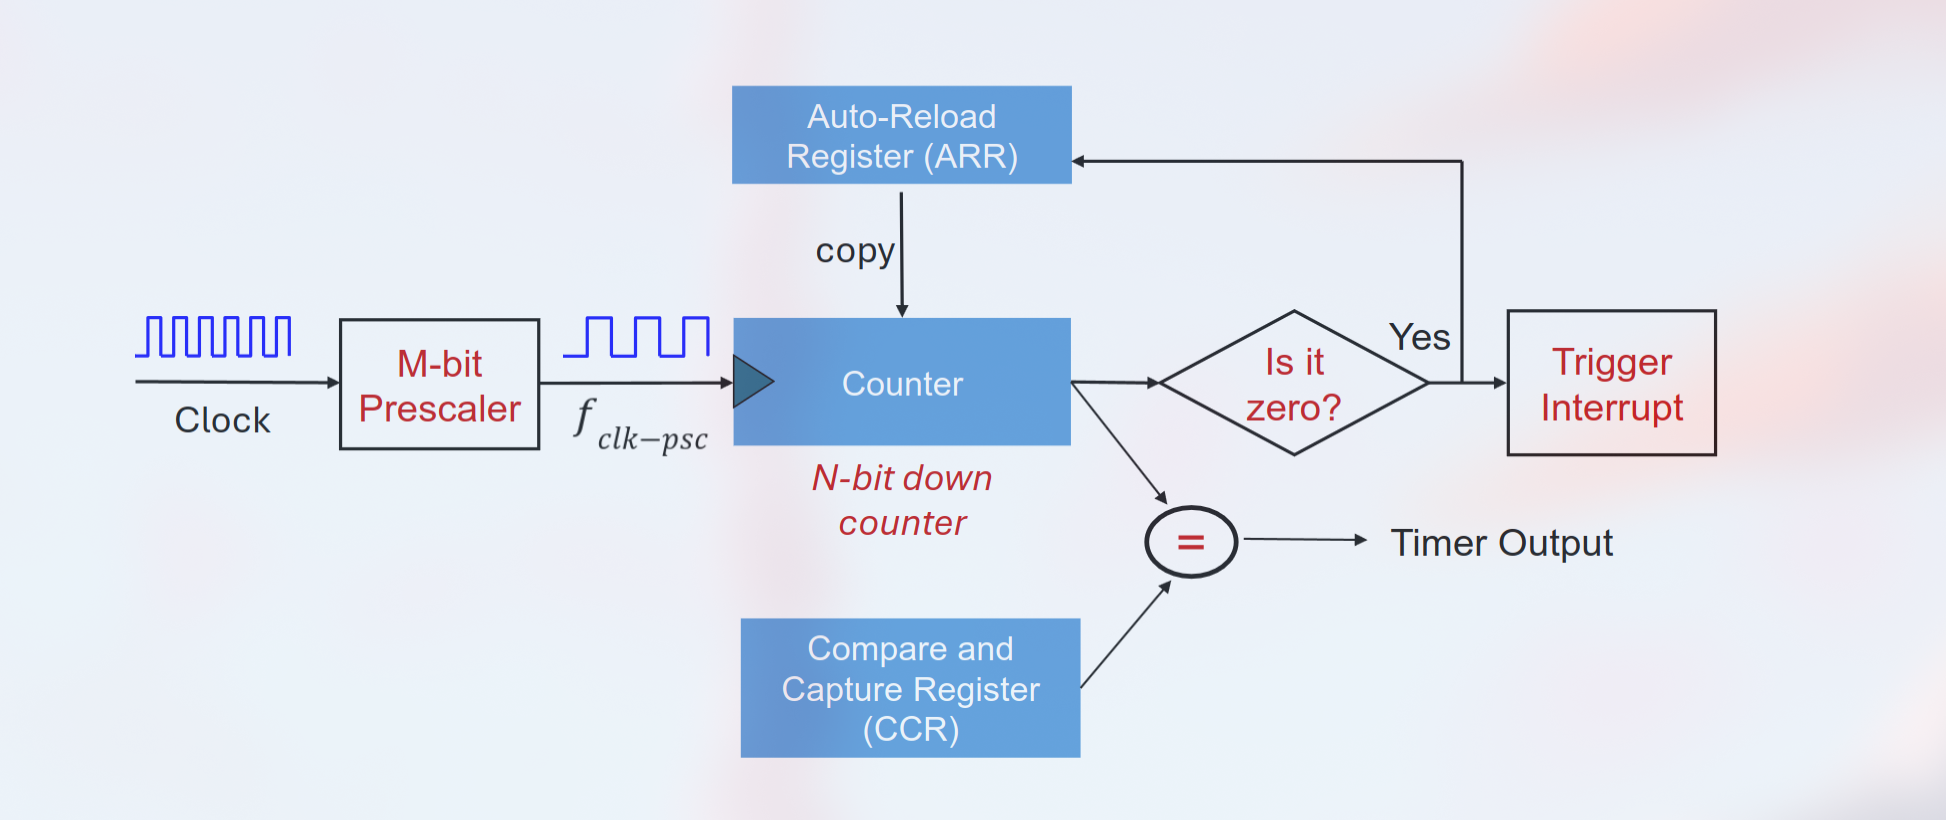
\includegraphics{images/outputmodetimer.png}
    \caption{Timer Output Mode}
    \label{fig:outputmodetimer}
\end{figure}

In general purposes timers, you can count down, up, or up and
down.

The output mode determines what happens when the CCR and counter
are equal. One output mode is active high. When the
timer value equals the CCR, then the timer output is set to high
and stays there. Another output mode is toggle, where the
output switches whenever the timer reaches the CCR value.

\emph{Pulse width modulation} (PWM) is a convenient way to
generate variable duty cycles. You just toggle the output
each time it reaches a given value of the CCR.
\begin{equation}
    \text{Duty Cycle} = \frac{\text{CCR}}{\text{ARR} + 1}
\end{equation}
\begin{equation}
    \text{Period} = (1 + \text{ARR}) \times \text{Clock Period}
\end{equation}
PWM outputs a digital waveform (i.e. either 0 or 1),
with a specific frequency and duty cycle.

We'd like to be able to have a DAC with a strong drive
strength like we have with GPIO.
We don't just want on/off states. We want multiple voltage levels.
Consider a square wave with a varying duty cycle:
We average the area under the curve.
The duty cycle of the wave is then the analog level.
We can average using a low-pass filter.
As long as the wave frequency is much higher than
the signal we want to model, no one will notice
the averaging. We can accomplish averaging with low-pass filters.
Each timer has a PWM mode where the output starts high, and goes low
when CNT == CCRx. The higher the duty cycle, the higher the average.
If the pulse frequency is much higher than that of the
desired signal, the noise will be imperceptible.
\section{Debouncing}

When a mechanical button is pressed, there is a
period where the signal is neither high nor low,
because of vibrations in the conducting plate it
connects or other non-ideal physical effects. This
is known as \emph{bouncing}, and it's rectified by
adding a Schmitt trigger and RC circuit to smooth
out the signal.

However, in real world systems we rarely have just one
button. We often have a matrix input, like a keypad.
Our Schmitt trigger setup doesn't work here, but
luckily a software solution exists. Set up the CPU
connected to the keypad to scan each key for being pressed.
It doesn't need to check constantly, just often enough that
it will catch a button press.

The work of scanning can be done incrementally using a timer interrupt.
On each interrupt, the ISR will:
\begin{itemize}
    \item read all the columns
    \item put the value read for each key of the current row into its own history byte
    \item turn off the voltage for the row
    \item turn on the voltage for the next row (for the next ISR invocation)
    \item return
\end{itemize}

The keys on a keypad can still bounce. Pressing and letting go of a
button may look something like \texttt{00000001001011111...1111101000000}.
In this example, the button bounces on press and release. However, the
history byte eventually stabilizes and is full of entirely \texttt{1}s
or \texttt{0}s. To detect a press or release, we search all the history
bytes that represent the keys. The first time we detect a change, like in
\texttt{00000001}, we say that is the start of a press or release. We say
the press or release is done when the history byte queue is back to only
one number.

We want to scan the keys faster than they can be pressed or released, but
slower than the total bounce time for any key. Say a button can bounce for
10ms, and we scan one row of the 4-row keypad every 1ms. Then when you
press the button, the instance you read a one, you do not know if the
input is stabilized. It could still bounce, since it has been 0ms.
The second time you read a bit, it could still be bouncing, since 4ms is
within the 10ms bounce time. The third time you read a bit, it could still
be bouncing, since it has only been 8ms. By the fourth bit you read, you are
certain it is a one.


\section{Multiplexing}

\emph{Multiplexing} is when you rotate through a task fast enough
that it gives the appearance of being simultaneous.
Key scanning is a specific example of input multiplexing and encoding.
Another example is driving displays. Turn on one SSD at a time.
Rotate through them rapidly enough that your persistence
of vision makes it appear they are all on simultaneously and displaying
different digits.

\end{document}